\chapter{Related Work}

This section outlines key findings of related work on gender bias in MT, with a focus on the English-German (EN-DE) language pair to build the theoretical knowledge base. The research aims are to (1) define the core concept of gender bias in MT, (2) establish the relevance of the topic, (3) identify the research gap, and (4) justify technical design choices. To support this, I examine datasets, model types, and tools used in previous studies.

For the literature review I combined incremental and conceptual literature review methods, where each source led to the identification of the next. Based on this progression, I identified key concepts and used them to organize and interpret the literature, aligning with a conceptual approach. The structure followed the qualitative Information Systems framework by \citet{schryenWritingQualitativeLiterature2015} and was further informed by \citet{shresthaExploringGenderBiases2022} and \citet{savoldiDecadeGenderBias2025}, who both conducted systematic reviews on gender bias in ML and MT respectively. 

\section{Literature Search Process}

\subsection{Search Sources and Tools}
Sources were primarily searched on \href{https://scholar.google.com/}{Google Scholar} and \href{https://www.perplexity.ai/}{Perplexity}, which served as an additional search engine. Prompts and outputs from Perplexity have been saved and are included in the appendix. To organize and manage the collected sources, \href{https://www.zotero.org/}{Zotero} was used throughout the process.

\subsection{Literature Review Framing}

To answer the four research aims, I have defined the key concepts in \autoref{tab:key-concepts}. Key search terms consisted of \textit{gender bias}, \textit{machine translation}, \textit{AI}, \textit{machine learning}, \textit{German}, \textit{stereotypes}, and \textit{detection}. The focus was on literature published between 2019 and 2025 to maintain relevance and currency, while foundational and definitional works from earlier periods were selectively included. The initial search for the term \textit{gender bias in machine translation} returned over 18,000 results. Through my iterative selection process, this was narrowed down to 34 core sources.

\renewcommand{\arraystretch}{1.3}
\begin{table}[ht!]
\centering
\begin{tabularx}{\textwidth}{>{\raggedright\arraybackslash}p{6.5cm}X}
\toprule
\textbf{Key Concept} & \textbf{Description} \\
\midrule

Foundations of Gender Bias in Natural Language Processing & Traces early research that identified gender bias in language. Focuses on foundational studies that showed why the issue matters and how later work builds on these findings. \\

Sources and Manifestations of Bias & Explains how stereotypes shape language and persist over time. Describes how societal bias enters training data, model design, and system feedback. Shows how bias appears in machine translation and everyday language. \\

Linguistic Challenges in English-German Translations & Explores key grammatical differences between English and German that affect translation. Focuses on how the lack of gender in English and its presence in German can lead to biased outputs. \\

Mitigation Strategies and Current Limitations & Reviews how current research tries to reduce gender bias in NLP. Highlights what these methods can and cannot do. Helps identify where a classification-based approach could fill gaps and improve bias detection in translations. \\

\bottomrule
\end{tabularx}
\caption{Key concepts relevant to this thesis}
\label{tab:key-concepts}
\end{table}


\subsection{Citation Tracking}
Backward citation searching involved reviewing references cited by selected papers, prioritizing frequently cited and foundational works relevant to gender bias in MT. Forward citation searching used Google Scholar's "cited by" function to identify newer research citing those key papers. Filtering with specific terms (e.g., \textit{German} and \textit{machine translation}) was applied during forward search to maintain focus. In addition to the main review process, supplementary sources were included as needed throughout the writing phase. These consist of contextual references, statistics, or secondary citations that support specific points but were not part of the core conceptual or methodological framework.

\subsection{Selection Criteria and Screening Process}\label{subsection:selection_criteria}
Titles and abstracts were manually screened to select relevant studies. \textbf{Inclusion criteria} required sources to specifically address gender bias in MT, provide examples or discussions of gender-related errors, or explain the significance of gender bias in this context. Sources also had to be available in full text without access restrictions. \textbf{Exclusion criteria} filtered out studies focusing on general NLP bias without a direct link to MT, non-gender biases, and highly technical papers lacking contribution to the general understanding of gender bias or that did not provide additional knowledge beyond what was already found in previously published papers. Full texts were reviewed after initial screening to confirm relevance and extract insights. Redundant sources not providing new perspectives aligned with the thesis goals were excluded.

\section{Foundations of Gender Bias in Natural Language Processing}

This section outlines why gender bias is a subject of research in the first place and where it connects to broader social and ethical questions. It first looks at early studies that brought attention to gender patterns in language technologies and raised awareness of their social impact. Understanding these origins helps explain why it continues to be relevant today.

\subsection{Foundational studies}
The existence of gender bias in MT is well-documented. First mentions of this issue date back to over a decade ago, having been recognized by a paper by \citeauthor{schiebingerScientificResearchMust2014} in 2014. Since then, there has been a general increase in research papers focusing on this topic, especially between 2019 and 2023 \citep{savoldiDecadeGenderBias2025}.

\textbf{\citet{pratesAssessingGenderBias2019}} conducted a large-scale quantitative study using Google Translate, translating sentences such as "He/She is an engineer" from twelve gender-neutral languages into English. The study revealed a significant overrepresentation of male pronouns, particularly in STEM-related occupations. This was not attributable to actual gender distributions in the labor market, suggesting that the bias stemmed from imbalances in the system’s training data. The paper received widespread media coverage, which was then followed by a policy change by \citeauthor{googleReducingGenderBias2018} to present both feminine and masculine official translations for ambiguous queries \citep{googleReducingGenderBias2018}, acknowledging that their model inadvertently replicated gender biases (see \autoref{fig:gt_prates_example}). 

Following that, \textbf{\citet{stanovskyEvaluatingGenderBias2019}} introduced \href{https://github.com/gabrielStanovsky/mt_gender}{WinoMT}, a challenge set designed to evaluate gender bias in translations of English sentences into eight target languages with grammatical gender. The study showed that both commercial and academic MT systems failed to preserve correct gender in non-stereotypical roles, while performing better on stereotypical ones. In line with the findings of \citeauthor{pratesAssessingGenderBias2019}, the study demonstrated a systematic preference for traditional gender roles in translations. This pattern is further supported by \textbf{\citet{choMeasuringGenderBias2019}}, who showed that occupational terms exhibit higher levels of gender bias across systems compared to other semantic categories. 

These foundational studies not only confirm the existence of systematic gender bias in MT outputs, but also lay the groundwork for subsequent research that builds upon their findings and approaches to develop more robust evaluation methods and mitigation strategies.

\subsection{Human-Centered Studies}
Not until half a decade later, studies have begun to assess the real-world implications of gender bias by measuring its impact on human effort. Before that, the human component has mostly been neglected. \citet{savoldiWhatHarmQuantifying2024} conducted a human-centered evaluation in which approximately 90 participants were tasked with post-editing MT outputs to ensure gender-accurate translations.

The study employed behavioral metrics such as time to edit and the number of edits, measured through human-targeted error rate, to quantify the effort required. The results showed that post-editing feminine translations required nearly twice as much time and four times the number of editing operations compared to masculine counterparts. Consequently this effort gap also translates into \textbf{higher economic costs}, suggesting a measurable \textbf{quality-of-service disadvantage that disproportionately affects women}. \citeauthor{savoldiWhatHarmQuantifying2024} concluded that current automatic bias metrics do not sufficiently capture these human-centered disparities, emphasizing the need for evaluation methods that reflect real user experience.

A comparison analysis between AI and human translations was conducted by \citet{smacchiaDoesAIReflect2024}. The study's aim was to understand if gender bias is still present in how people think in society. Their results demonstrated a consistency between the outcomes generated by the AI tools and the human survey responses, suggesting that \textbf{AI tools reflect human behaviour} regarding job occupations and gender distributions in society. They also identified a "converging bias", which is a tendency to maintain consistency in the output based on an initial translation. For example, if the \textit{doctor} in \textit{"The doctor arrived"} is translated with a male form, the subsequent input \textit{"The doctor then started working"} is likely to be translated as male too.


\section{Sources and Manifestations of Bias}

To address a problem, one needs to understand its origins. This section outlines how societal bias transfers into data and NLP systems. It looks at different types of bias, with a focus on those that shape model behaviour and outputs.

\subsection{Types of Technical Bias}
Technical bias happens when limitations in the system's design affect how models learn and make predictions \citep{stanczakSurveyGenderBias2021}. This includes the way data is processed or how the model handles information.

\citet{shahPredictiveBiasesNatural2020}, as described by \citet{ullmannGenderBiasMachine2022}, differentiates between four technical origins of biases:

\begin{itemize}
    \item \textbf{Selection Bias:} Happens when the training data does not reflect the context in which the model is used (e.g., using Wikipedia data for detecting harmful language on Twitter).
    
    \item \textbf{Label Bias:} Occurs when annotations in the dataset are incorrect or skewed. This can be influenced by the annotators' own biases or lack of awareness of diverse linguistic expressions.

    \item \textbf{Model Overamplification:} During training, models can exaggerate patterns found in the data. This is the cause of the aforementioned "only women cook" example (see \autoref{subsection:implications_of_gb_in_nlp}).

    \item \textbf{Semantic Bias:} Stems from associative relationships within the data, where certain words or phrases are frequently co-occurring with specific genders (e.g., "he" with "doctor").
\end{itemize}

\subsection{Human Bias Transfer}
Stereotypes and gender roles stem from historical and cultural perceptions of men's and women's societal roles, many of which are obsolete but still influential. For example, when men and women often take on different roles at work and at home, it shapes how people think about their personalities and qualities. \textbf{Correspondence bias} can emerge, where people infer attributes from observable behaviours \citep{godsilEffectsGenderRoles2016}. It is a result of the human brain's automatic categorization of stimuli when faced with incomplete information, often a quick and unconscious process. Common groupings are gender, race and age. These associations can be reinforced by popular media, such as TV and advertisements \citep{godsilEffectsGenderRoles2016}, just as much as it can be influenced by modern technology like MT tools. 

Similarly to how humans are shaped by their environemnt, ML models learn from data they are trained on. \textbf{Biases are thus reflected and reinforced in the final models} \citep{stanczakSurveyGenderBias2021,smacchiaDoesAIReflect2024}. That bias can, again, reflect back to humans and create a regressive feedback loop \citep{barclayInvestigatingMarkersDrivers2024a,shresthaExploringGenderBiases2022}. LLMs like GPT-3 were trained on hundreds of billions of words, making it practically impossible to review all of the data, therefore allowing misinformation or offensive content to be reproduced by the system.

\citet{ullmannGenderBiasMachine2022} notes that the scale of training data (e.g., 175 billion parametres for GPT-3) makes it practically impossible to review all of it, allowing misinformation or offensive content to be reproduced by the system. The author also points out that platforms like Wikipedia and Reddit are male-dominated and often contain harmful or false content, which contribute to gender bias.

\subsection{Common Gender Bias Phenomena}
While the previous sections discussed the sources of gender bias, this section focuses on how such biases appear in MT outputs. Drawing on selected studies, I identify recurring patterns of bias and group them into thematic categories. An overview of the result is prestented in \autoref{tab:gender_biases}. It is important to note that, due to the complex nature of gender bias, clear boundaries between these categories are not always possible. Definitions in the literature often overlap, and some patterns may extend or intersect with others. The classification presented here reflects my synthesis of the existing research, aiming to provide a structured framework for analysis despite these inherent ambiguities.

\subsubsection{Stereotype-driven bias}

The majority of gender bias mentioned fall into stereotype-driven categories. Most notably, the persistent use of the \textbf{generic masculine} as default (see subsection \ref{subsection:generic_masculine}) and systematic \textbf{occupational stereotyping}. When translating gender-neutral terms, most systems overwhelmingly favor masculine forms, e.g., translating "doctor" to masculine forms like "el médico" (Spanish) or "der Arzt" (German) even in neutral contexts \citep{smacchiaDoesAIReflect2024,choMeasuringGenderBias2019,pratesAssessingGenderBias2019}. This bias becomes particularly evident in professional contexts, where translation outputs closely mirror societal stereotypes rather than linguistic requirements. \citet{smacchiaDoesAIReflect2024} found that across major commercial systems including Microsoft Azure, DeepL, and Google Translate, male-dominated occupations were translated using masculine forms in \textbf{94\%} of cases.

Stereotype-driven bias extends beyond occupational terms. As demonstrated by \citet{pratesAssessingGenderBias2019}, adjective associations exhibit similar gendered patterns. "Shy" or "desirable" disproportionately trigger feminine pronouns, while "guilty" or "cruel" default to masculine forms. These associations occur independently of professional contexts, revealing deeper linguistic biases embedded in translation systems.

\subsubsection{Contextual analysis} \label{subsection:contextual_analysis}

Current MT systems exhibit fundamental limitations in handling gender context, particularly when compared to human translation capabilities. Where professional translators successfully interpret both linguistic markers (pronouns, grammatical agreements) and extra-linguistic knowledge (cultural norms, real-world contexts) to determine gender \citep{rescignoGenderBiasMachine2023}, automated systems struggle with consistent implementation.

\textbf{Coreference resolution} is the technical process that should leverage contextual cues for gender. In translation, this helps systems use the right gender based on context. But as shown by \citet{choMeasuringGenderBias2019}, many systems still struggle with this, especially when the gender is mentioned earlier in the text or in another sentence. Datasets like WinoMT \citep{stanovskyEvaluatingGenderBias2019} show that translation models often miss these links and ignore gender cues, leading to biased results.

Sometimes models even actively disregard \textit{explicit} gender markers in the immediate sentence. For example:
\begin{itemize}
    \item "The doctor asked the nurse to help \textbf{her}" $\rightarrow$ incorrectly translated with masculine "el doctor" (Spanish) despite the feminine pronoun.
    \item "The doctor finished \textbf{her} shift" $\rightarrow$ rendered as masculine "der Arzt" (German) by Google Translate \citep{stanovskyEvaluatingGenderBias2019}
\end{itemize}

\begin{table}[ht]
\centering
\begin{tabularx}{\textwidth}{>{\raggedright\arraybackslash}p{3cm} >{\raggedright\arraybackslash}X >{\raggedright\arraybackslash}X}
\toprule
\textbf{Bias Type} & \textbf{Definition} & \textbf{Example} \\
\midrule
\multicolumn{3}{l}{\textbf{Stereotype-Driven Biases}} \\
\midrule
Occupational Stereotyping & Gender assigned to occupations based on societal stereotypes rather than context & "Engineer" → masculine; "nurse" → feminine, regardless of source \\
\addlinespace
Beyond Occupations & Gender bias appears in adjective associations and other non-professional contexts & Shy/desirable" → female pronouns; "guilty/cruel" → male pronouns \\
\addlinespace
Generic Masculine & Masculine form used by default in gender-ambiguous cases & "The students are late" → "Die Studenten (m) sind zu spät". translated as male, even when gender is unclear \\
\midrule
\multicolumn{3}{l}{\textbf{Contextual Failures}} \\
\midrule
Coreference Resolution Failures & MT fails to track gender associations across sentences/phrases & "Anna is a teacher. \textbf{She} teaches math." → "teacher" translated as male \\
\addlinespace
Ignoring Contextual Cues & MT actively disregards explicit gender markers in the immediate context & "She is a baker" → translated as male baker \\
\bottomrule
\end{tabularx}
\caption{Summary of common gender bias manifestations in MT systems.}
\label{tab:gender_biases}
\end{table}


\subsection{Implications of Gender Bias in Natural Language Processing} \label{subsection:implications_of_gb_in_nlp}
As outlined in \autoref{section:social_and_ethical_importance_of_addressing}, this section builds on the social and ethical foundations by examining how gender bias in NLP can lead to the amplification of existing social biases \citep{rescignoGenderBiasMachine2023}.
\citet{ullmannGenderBiasMachine2022} illustrates this with an example: if a dataset predominantly associates cooking with women, the system may amplify this pattern, reinforcing the assumption that cooking is an activity exclusive to women. This not only reproduces but also strengthens a social stereotype, potentially resulting in \textbf{representational harm}, namely, the continued spread of reductive or biased portrayals of a particular gender \citep{stanczakSurveyGenderBias2021}. 

This also contributes to the invisibility of women in professions traditionally dominated by men \citep{kapplAreAllSpanish2025}. Studies show that gender bias in machine-generated text, such as children's stories or job advertisements, can \textbf{influence how young people view themselves} \citep{soundararajanInvestigatingGenderBias2024,kapplAreAllSpanish2025}. It may shape their interests, hobbies, and decisions about education and careers. This effect is especially noticeable in Science, Technology, Engineering, and Mathematics (STEM) fields \citep{pratesAssessingGenderBias2019}, where stereotypes are more deeply rooted. When job descriptions or mock interviews use gender-exclusive pronouns, women report feeling less sense of belonging, lower motivation, and weaker identification with the role \citep{godsilEffectsGenderRoles2016}. As a result, they may self-select out of the application process, reducing the pool of female talent available to employers and \textbf{reinforcing existing gender gaps in the workforce}.

On the other hand, research shows that using gender-inclusive language, e.g. "she and he" or "one", can lead to more positive reactions from women when considering job opportunities. It helps reduce stereotype threat and improves how women perceive and engage with different environments \citep{ godsilEffectsGenderRoles2016}. Hence, complying with gender-inclusive langauge may offer companies both social and competitive advantages.


\section{Linguistic Challenges in English-German Translation}

Because this thesis focuses on EN-DE translation, we need to take a closer look at how gender works in German. This section will explore the main linguistic features that affect gender expression in German. Then, it will review key studies that examine how these features influence bias in translation.

\subsection{Grammatical Gender}
Although both English and German originate from the Indo-European language family \citep{baldiEnglishIndoEuropeanLanguage2008}, they have different characteristcs. English does not assign grammatical gender to nouns. The article "the" is used universally, independent of what it refers to. On the contrary, German assigns one of three grammatical gendered articles to nouns: "der" (m), "die" (f) and "das" (n). The form or ending of a noun may also change depending on its grammatical gender. While English has a few gendered word pairs, such as "actor" (m) and "actress" (f), gender distinctions in German apply broadly across the entire noun system. "Der Student" refers to a male student, whereas "die Studentin" refers to a female student. Note that grammatical gender has no connection to societal or biological gender. It is a rule of the language rather than a reflection of identity. For example, the German word Mädchen (girl) is grammatically neuter and takes the article "das". This is not because the referent lacks gender, but because the suffix "-chen" automatically assigns neuter gender. This illustrates that grammatical gender in German follows structural rules, even when they contradict real-world gender associations.

\subsection{Gender-Fair Language}

\subsubsection{The Generic Masculine} \label{subsection:generic_masculine}
In both singular and plural contexts, the \textit{generic masculine} refers to the default use of the masculine grammatical gender. It is commonly used in spoken German \citep{lardelliBuildingBridgesDataset2024,schmitzGermanAllProfessors2022}, although research has consistently shown that the generic masculine creates a male bias in mental representations, leading readers or listeners to think more of male than female examples \citep{sczesnyCanGenderFairLanguage2016}. Similarly, \citet{rescignoGenderBiasMachine2023} observed a predominance of masculine forms in translation outputs (approximately 90\% in Google Translate and 85–88\% in DeepL for EN-IT and EN-DE), even when the original sentences contained relatively few masculine references. These linguistic biases in human language naturally carry over into ML systems. Since most models for NLP are trained on large datasets of human-generated text, they inadvertently learn and reproduce the same sociolinguistic biases present in the data \citep{choMeasuringGenderBias2019}.

\subsubsection{All students are male}
The English sentence "The students are studying" does not indicate the genders of the individuals involved. There are various ways to translate that sentence into German. The plural forms of the gendered term "student" would be "die Studenten" (multiple male students) and "die Studentinnen" (multiple female students). The problem arises when there is a mix of male and female students or when the genders are unknown. 
Using the common generic masculine, the sentence translates to \textit{die Studenten lernen}, with the male term referring to a (potentially mixed-gender) group. As \citet{schmitzGermanAllProfessors2022} pointed out, if the female form is not explicitly mentioned, the phrase is understood as all students are male.

The rise of the gender-fair language (GFL) debate was a response to this structural asymmetry. It refers to the use of language that treats all genders equally and aims to reduce stereotyping and discrimination \citep{sczesnyCanGenderFairLanguage2016}. 
There are four main approaches to GFL in German identified by \citet{lardelliBuildingBridgesDataset2024}. I will not discuss two of them further because they are less common and face greater hurdles for broader public and professional acceptance.

\begin{itemize}
    \item \textbf{Gender-neutral rewording:}  
    This uses neutral terms instead of gendered nouns, e.g., \textit{die Studierenden lernen}. A challenge for this version is that neutral alternatives do not exist for every noun and cannot be consistently applied.

    \item \textbf{Gender-inclusive characters:}  
    This combines masculine and feminine forms using a character like \textit{*}, \textit{:}, or \textit{\_}, e.g., \textit{die Student*innen lernen}. This method is consistent but may interrupt reading flow and lacks standardization.
\end{itemize}

\noindent Another approach not mentioned by \citeauthor{lardelliBuildingBridgesDataset2024} is to simply name both forms (pair form), e.g., \textit{die Studenten und Studentinnen lernen}. It is currently the most used GFL form in German \citep{waldendorfWordsChangeIncrease2024}, briefly surpassing the star and colon characters as seen in \autoref{fig:gfl_types_frequency}.

\begin{figure}
	\centering
		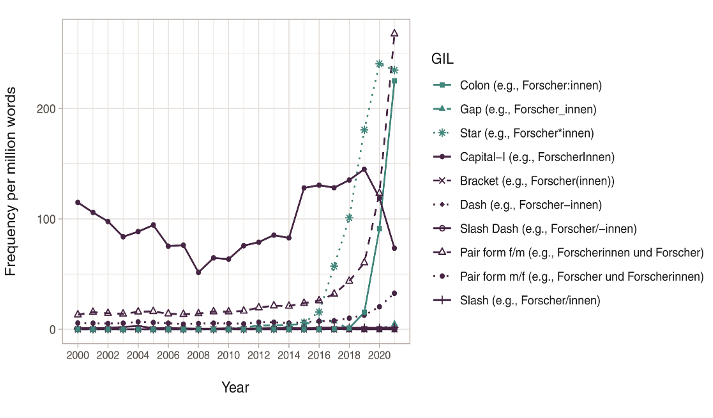
\includegraphics[width=1\textwidth]{gfl_types_frequency.png}
	\caption{Frequency of different types of gender-inclusive language. Source: \citet{waldendorfWordsChangeIncrease2024}.}
	\label{fig:gfl_types_frequency}
\end{figure}


\subsection{English-German Studies}
This language pair in particular is sparsely analysed in academia. I found \textbf{four relevant papers about gender bias in EN-DE MT} that fit my inclusion criteria defined in chapter \ref{subsection:selection_criteria}. Some other sources include German among multiple target languages (e.g., \citeauthor{stanovskyEvaluatingGenderBias2019}'s foundational study), but these do not provide detailed analysis specific to German. Therefore, I do not consider them EN-DE focused sources. The following studies provide a closer look at gender bias specifically in this language pair.

\textbf{\cite{ullmannGenderBiasMachine2022}} performed a corpus-linguistic analysis of training data, meaning they studied large collections of text to identify patterns and structures related to gender bias. The dataset consisted of 17.2 million sentence pairs sourced from \href{https://commoncrawl.org/}{\textit{Common Crawl}}. They then tested different techniques to reduce gender bias in a MT system trained on that corpus. Their findings support the broader patterns discussed in this thesis: masculine forms dominate by default, gender stereotypes shape translations, and professions are translated in line with societal roles. Their key contribution lies in testing mitigation strategies. They show that fine-tuning with a small, gender-balanced dataset can reduce bias in MT outputs. 

\textbf{\citet{rescignoGenderBiasMachine2023}} evaluated gender bias in Google Translate and DeepL for EN-IT and EN-DE using the \href{https://github.com/amazon-science/machine-translation-gender-eval}{MT-GenEval} dataset. They focused on how often professions were translated with male or female forms, both with and without gender-revealing context. Without context, both systems defaulted strongly to masculine forms (over 85\%) for both languages. Contextual information generally improved alignment with reference translations, but in a few cases, context led to incorrect gender disambiguation that had not occurred without it. This suggests that contextual cues can occasionally misguide the system rather than improve performance. The authors also noted that most users are unaware of gender bias, especially if they lack fluency in the source language. Currently there is no system in place to inform them when biased translations occur.

\textbf{\citet{lardelliBuildingBridgesDataset2024}} created a \href{https://github.com/g8a9/building-bridges-gender-fair-german-mt}{Gender-Fair German Dictionary} that includes professions and common nouns for people. They tested several MT systems and evaluated translations from Wikipedia and parliamentary texts. Translations were manually annotated as masculine, feminine, gender-neutral, or gender-inclusive. They also used zero-shot detection with GPT models, where GPT tries to identify gender fairness without specific training. Results showed strong masculine bias and poor automatic detection of GFL, requiring human review and therefore proving zero-shot detection to be challenging. Unlike most research focusing on professions, this study covers a broader range of terms.

\textbf{\citet{kapplAreAllSpanish2025}} introduced \href{https://github.com/michellekappl/mt_gender_german}{WinoMTDE}, a German gender bias evaluation test set based on \citealp{stanovskyEvaluatingGenderBias2019}'s WinoMT. It contains 288 balanced German sentences with clearly gendered subjects and tests occupational stereotyping in MT from German to other gendered languages. The study found that gender bias persists due to model architecture and training data, not source language ambiguity. Major limitations of the study include the small dataset size and broad occupation categories. It also misses some bias types and faces alignment issues affecting accuracy estimates. They call for future researchers to expand the dataset, improve annotations and include diverse gender terms. This study's evaluation pipeline is the most advanced among EN–DE studies for automated bias detection.

\subsection{Cross-Language Perspectives}
Gender bias in MT is not limited to English and German. Many other language pairs show similar patterns, revealing how bias is shaped by both language and the systems behind it. This section includes a few examples from other languages to show that the issue is not specific to German in order to keep the broader context in mind and avoid a narrow, language-specific perspective.

Some studies looked at \textbf{back-translation from English through gender-neutral languages} like Finnish, Indonesian, and Turkish, then back to English. They found different pronoun patterns depending on the language. This shows why it is important to study many languages to understand gender bias better. Verbs played a big role in how gender was inferred in translations. New metrics, like Adjusted Uncertainty, helped capture these details. Some translation systems showed signs of reducing bias over time \citep{barclayInvestigatingMarkersDrivers2024a}.

When translating \textbf{gender-neutral Korean into English}, MT systems often leaned toward masculine pronouns. This happened because the training data had more male examples. Some systems made technical changes that sometimes favored feminine forms, which suggests bias mitigation is possible, however ideally, translations should stay neutral or balanced \citep{choMeasuringGenderBias2019}. \textbf{Japanese and Chinese} demonstrated exceptionally low percentages of female pronouns in translations, going as low as 0.196\% for Japanese and 1.865\% for Chinese \citep{pratesAssessingGenderBias2019}.

Even when translating \textbf{between languages that both use grammatical gender}, like German and Spanish, Ukrainian, or Russian, gender bias still shows up \citep{kapplAreAllSpanish2025}. This goes against the assumption that clear grammatical cues would reduce ambiguity and help systems make better choices. Instead, the bias often stays or even gets worse, suggesting that the problem is not just about language structure but also how MT systems learn and generalize from data.

Most studies focus on English paired with another Western language, with only a few exceptions including West or East Asian languages. This adds an Anglocentric bias to the existing gender bias problem \citep{savoldiDecadeGenderBias2025}.


\section{Mitigation Strategies and Current Limitations}    

Different approaches have been tested to mitigate gender bias in MT. Despite of various proposals, no single solution has emerged as definitively superior \citep{savoldiDecadeGenderBias2025}. The following section gives an overview of these strategies, takes a closer look at one selected approach, and highlights key limitations in current research.

\subsection{Technical Mitigation Approaches}
\citet{savoldiDecadeGenderBias2025} recently grouped the mitigation approaches suggested in the past decade of research about gender bias in MT. 

A common focus is to create new test sets or ways to measure bias in MT. Instances of these are WinoMT, MT-GenEval and GeNTE. They serve the purpose of determining the extent of gender bias present. Usually these approaches incorporate statistical evaluations or bias metrics, which can then be used for actual mitigation / detection systems. A few papers compare different MT systems or add additional types of input like a document level approach or image guided MT. It tests whether changing the system's structure and/or adding more context can reduce gender bias. However, as previously stated in subsection \ref{subsection:contextual_analysis}, many systems still struggle with coreference resolution.

Stepping inside the realm of LLMs, zero-shot detection has been deployed to automatically evaluate outputs regarding gender bias. Zero-shot in this case is the prompting of GPT models to identify gender bias in the translated text without providing specific examples nor fine tuning the models. The findings suggest that the technology is not yet ready to reliably detect biased or neutral instances without human oversight \citep{lardelliBuildingBridgesDataset2024}. 

Furthermore, by extending the reserach of \citet{tomalinPracticalEthicsBias2021}, \citet{ullmannGenderBiasMachine2022} concerned herself with the pre-processing of data. The approach is to manipulate the training data \textit{before} it is fed into a ML model. This again can be divided into three strategies: (1) Downsampling, which removes data until the ratio of gendered terms is balanced, (2) Upsampling, which duplicates data to balance the ratio of gendered terms and (3), Counterfactual Augmentation by introducing opposite sentences of the under-represented terms. For example, if one corpus contains "He is a doctor", the counterfactual sentence "She is a doctor" would be added \citep{ullmannGenderBiasMachine2022}. All of the three strategies led to substantially worse translation performances. It has been proven that the implementation of pre-processing is not feasible if the overall translation quality is significantly compromised.

Generally, all solutions operate in a narrow area, not across all languages, types of biases and systems. This again proves the sheer difficulty of finding a fix to such a multifaceted issue spanning multiple disciplines. One approach, however, has shown more promise than others in balancing bias mitigation and translation quality: model adaptation.

\subsection{Model Adaptation as a practical solution}
Model adaptation (or domain adaptation) is the fine-tuning of a MT system \textit{after} it has been trained. It was introduced as a response to the pre-processing approaches yielding subpar results \citep{tomalinPracticalEthicsBias2021}.

This technique, as described by \citet{tomalinPracticalEthicsBias2021}, makes use of a small gender-balanced dataset called "Tiny", containing 388 sentence pairs which were either profession-based or adjective-based. The structures of the sentences are simple and follow the following scheme: \textit{"The [PROFESSION] finished [his/her] work"} or \textit{"The [ADJECTIVE] [man/woman] finished [his/her] work"}. In order to prevent "catastrophic forgetting", a result in which the model loses its performance on the original data while learning from the new dataset, Elastic Weight Consolidation (EWC) was applied. It helps the model maintain its general translation quality while still working towards the reduction of gender bias.

This approach is particularly effective because manually removing biases from massive corpora is far too computationally intensive and unsustainable to be a reasonable solution. In contrast, model adaptation requires only a small, curated dataset, making it a more feasible and scalable solution worth further investigation.

\subsection{What counts as fair?}

One major limitation is that gender bias is not yet fully discussed in society or in language studies, so there is \textbf{no agreed standard for gender-fair language} (GFL) \citep{lardelliBuildingBridgesDataset2024, savoldiDecadeGenderBias2025} and "fairness" heavily depends on personal views, culture, and context. Generally said, bias lies on a spectrum and changes with the chosen definition. Some argue that removing all biases is impossible \citep{ullmannGenderBiasMachine2022}; which, for instance, leads to questions about group fairness and individual fairness. Group fairness seeks to achieve the same statistics for all groups. Individual fairness aims for similar treatment of similar people. For example, in hiring, group fairness might enforce equal hire rates for men and women. Individual fairness might enforce equal chances for two equally qualified applicants, regardless of gender. These aims can conflict, where many settings cannot satisfy both at once. 

Due to the unclear definition in academia, I have to define what I consider fair to set a clear direction. In this thesis, I focus on reducing harmful bias rather than chasing a fully unbiased state. I deem fair \textbf{a system that does not predict gender incorrectly when the correct gender is clear}. This choice guides my work.

Further challenges are ethical and linguistic considerations, which I will not further elaborate in this section. See more under %ref to limitations of my own research chapter.
